\chapter{Описание предложенного алгоритма}

\section{Предобработка текста}
Предварительная предобработка текста состоит из следующих этапов:

\begin{enumerate}
	\item Токенизация текста - из документа (сообщения/отзыва) получаем последовательность слов (токенов). Осуществляется посредством библиотеки \texttt{NLTK}\footnote{https://www.nltk.org/}.
	\item Лемматизация слов - приведение слов к их леммам для сокращения словаря. Осуществляется посредством библиотеки \texttt{PyMorphy2}\footnote{https://pymorphy2.readthedocs.io/}.
	\item Векторизация слов - сопоставления словам плотных векторов фиксированной размерности. Используется предобученный на русскоязычном корпусе из социальных медиа \texttt{Word2Vec}\footnote{http://mlcourse.at.ispras.ru/}. Векторное пространство слов имеет размерность 300.
	\item Zero-padding - дополнение последовательностей векторов нулевыми векторами до заданной максимальной длины последовательности, зависящей от выборки.
\end{enumerate}

Полученное представление документа в виде последовательности слов-векторов будет далее подаваться на вход рекуррентной нейронной сети.

%-----------------------------------------------------
\section{Рекуррентная нейронная сеть}
Ключевой компонентой алгоритма решения поставленной задачи является однослойная двунаправленная рекуррентная нейронная сеть~\cite{schuster} типа GRU~\cite{cho}. GRU (Gated Recurrent Unit) может быть описан следующими уравнениями:
	\begin{align}
	z_{t}&=\sigma_{g}(W_{z}x_{t}+U_{z}h_{t-1})\\
	r_{t}&=\sigma_{g}(W_{r}x_{t}+U_{r}h_{t-1})\\
	\tilde{h}_{t}&=\tanh(Wx_{t}+U(r_{t}\circ h_{t-1}))\\
	h_{t}&=(1-z_{t})\circ \tilde{h}_{t}+z_{t}\circ h_{t-1}
	\end{align}	
где $x_{t}$ -- t-ый элемент последовательности, а $h_{t}$ -- внутреннее состояние сети в t-ый момент времени (после обработки $x_{t}$).

Входная последовательность подается на вход одной рекуррентной сети прямым порядком и другой сети - обратным. После чего выходы этих двух слоёв конкатенируются, образуя выходную последовательность $y_{t} = \left[\overrightarrow{h_{t}},\overleftarrow{h_{t}}\right]$. Таким образом строится двунаправленная рекуррентная сеть, архитектура которой изображена на Рисунке~\ref{fig:birnn}.

\begin{figure}[H]
  \centering
  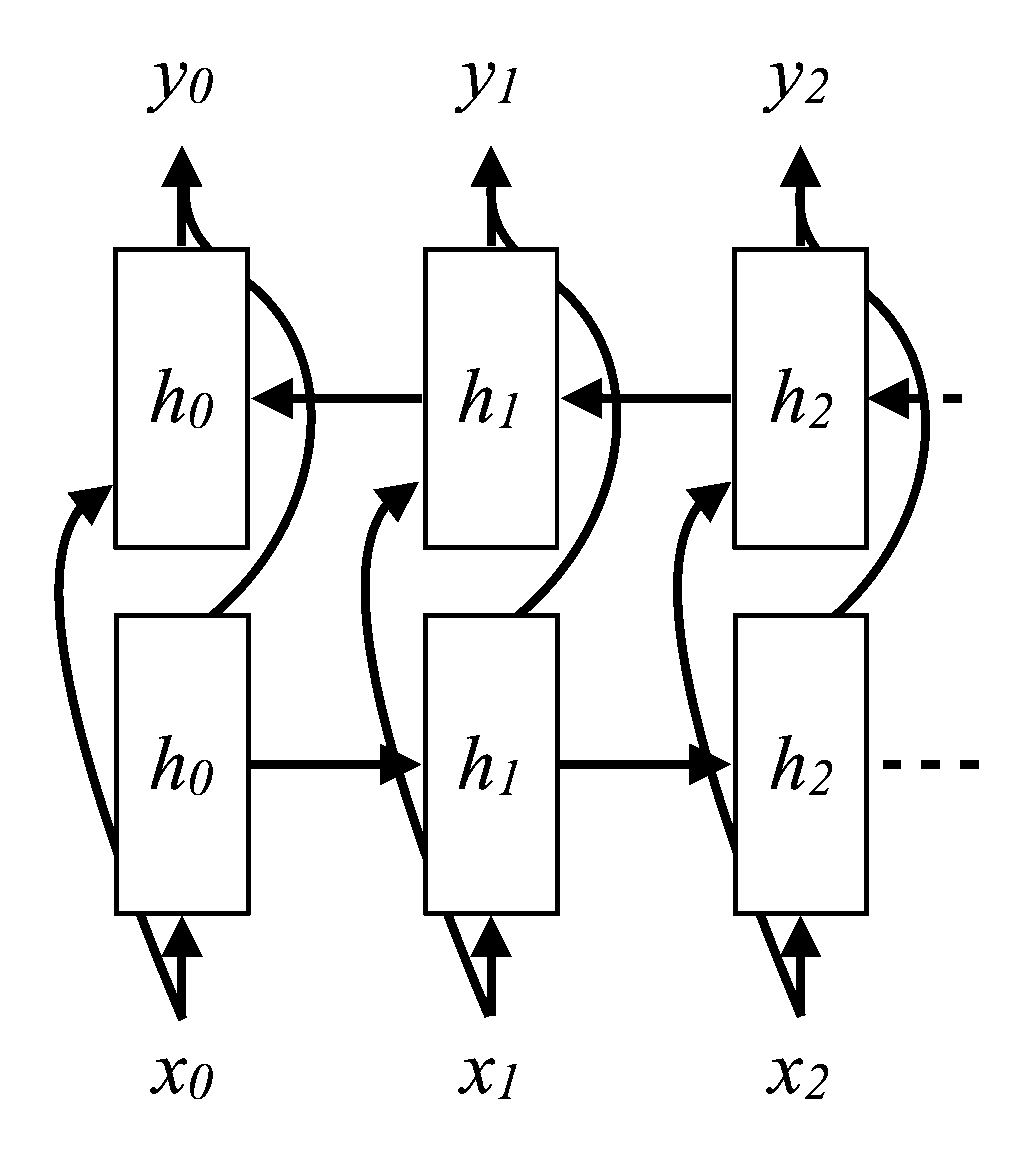
\includegraphics[width=0.5\textwidth]{images/birnn2_bin.png}
  \caption{Двунаправленная рекуррентная нейронная сеть}
  \label{fig:birnn}
\end{figure}
%-----------------------------------------------------
\section{Механизм внимания}
Классическим подходом к работе с выходом рекуррентной нейронной сети - $y_{1} ,..., y_{T} $ является рассмотрение лишь последнего вектора $y_{T}$, где $T$ -- длина входной (и выходной) последовательности, т.к. он аккумулирует в себе извлеченную информацию из всей входной последовательности. Рассматриваемый же нами подход -- механизм внимания~\cite{bahdanau} -- утилизирует все выходные векторы $y_{t}$, вычисляя их линейную комбинацию с коэффициентами $\alpha_{t}$, которые обучаются вместе с остальной сетью. Уравнения механизма внимания выглядят следующим образом:
	\begin{align}	
    \upsilon_{t}&=\tanh{(W_{\omega}y_{t}+b_{\omega})}\\
	\alpha_{t}&=\frac{\exp{(\upsilon_{t}^{T}u_{\omega})}}{\sum_{j=1}^{T}\exp{(\upsilon_{j}^{T}u_{\omega})}}\\
	\upsilon&=\sum_{t=1}^{T}\alpha_{t}y_{t}
	\end{align}	
Архитектура двунаправленной рекуррентной нейронной сети с механизмом внимания представлена на Рис.~\ref{fig:att}. Во время обучения к выходу слоя механизма внимания $\upsilon$ применяется регуляризатор Dropout~\cite{srivastava} для уменьшения переобучения.

\begin{figure}[H]
  \centering
  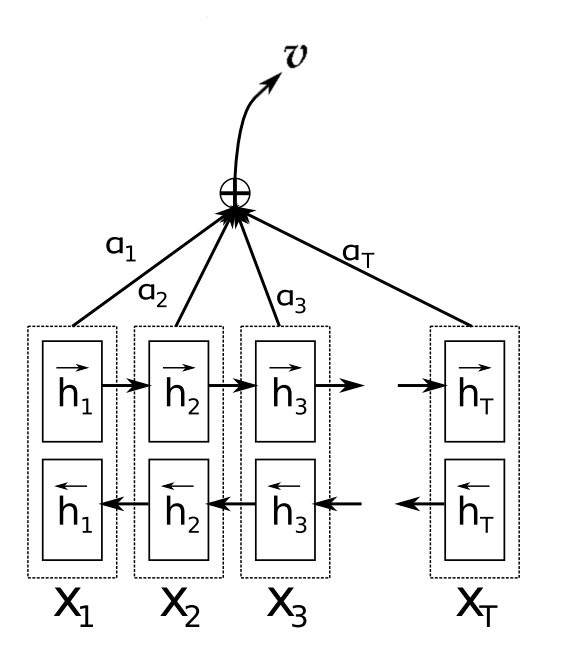
\includegraphics[width=0.5\textwidth]{images/att_edited.png}
  \caption{Двунаправленная рекуррентная нейронная сеть с механизмом внимания}
  \label{fig:att}
\end{figure}
%-----------------------------------------------------
\section{Полносвязанный слой}
После слоя механизма внимания следует полносвязный слой с функцией активации $softmax$, переводящий вектор $\upsilon$ в двух или трёхмерное пространство (в зависимости от числа классов в выборке), где каждое из чисел обозначает вероятность принадлежности объекта к соответствующему классу:
	\begin{align}	
    \hat{s}&=(\hat{s}^{(-1)},\hat{s}^{(0)},\hat{s}^{(1)})=softmax(W\upsilon+b)
	\end{align}
%-----------------------------------------------------
\section{Обучение}
Классификатор обучается при помощи метода оптимизации Adam и обратного распространения, минимизируя перекрёстную энтропию между выходным распределением $\hat{s}$ и истинным $s$:
    \begin{align}
    L(W)=-\sum_{i=1}^{n}\sum_{c\in\left \{ -1,0,1 \right \}}s_{i}^{(c)}\log{\hat{s_{i}}^{(c)}},
    \end{align}
Параметры модели подбираются по сетке при помощи перекрёстной валидации.
